
Filesystem in Userspace (FUSE) provides a relatively simple means to export a view to data as a virtual file system, but without the need for special privileges associated with similar techniques. FUSE is thus a popular choice to achieve legacy support for applications that require POSIX-like access semantics.


%%%%%%%%%%%%%%%%%%%%%%%%%%%%%%%%%%%%%%%%%%%%%%
\subsection{Logical View}

\begin{figure}
	\centering
	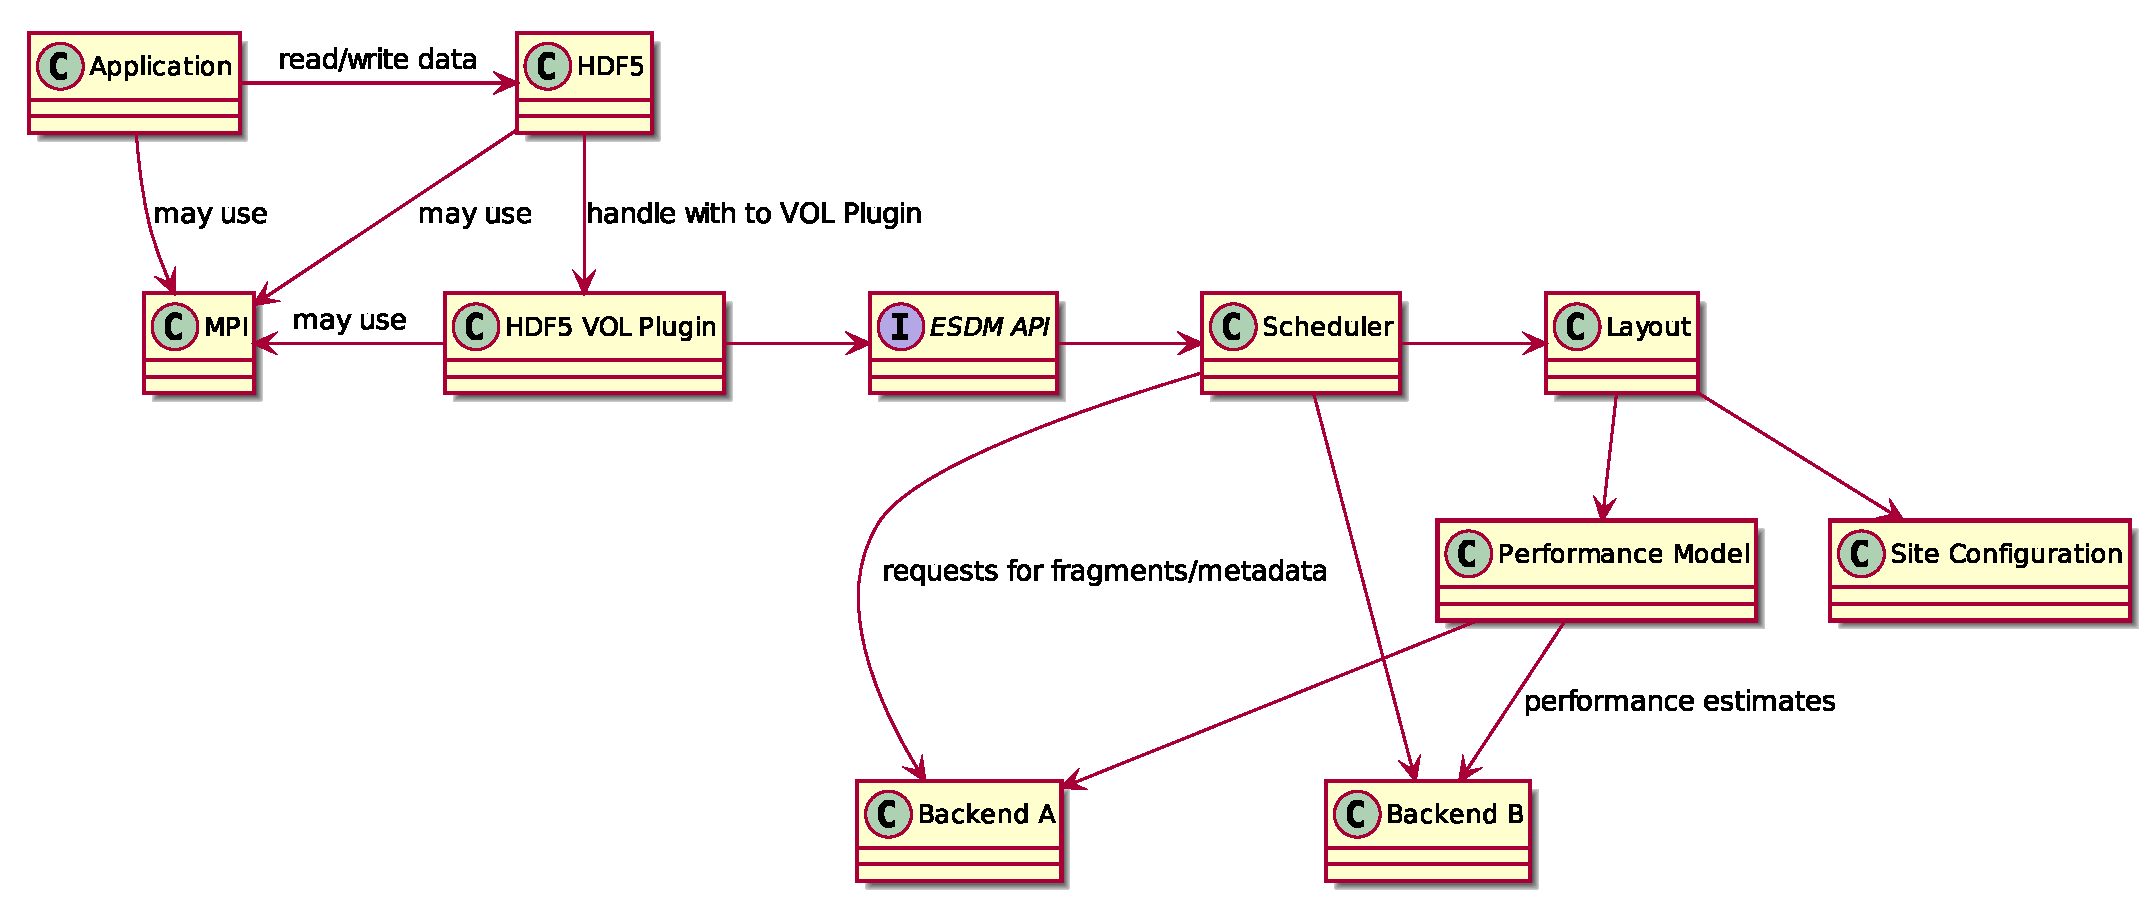
\includegraphics[width=0.5\linewidth]{esdm-fuse/logical.eps}
	\caption{Based on a FUSE ESDM configuration different views to data are possible. HDF5 files maybe created as soon as a job is known or on the fly.}
	\label{fig:esdm fuse logical view}
\end{figure}

Compatibility to legacy applications is the primary motivation to provide an ESDM FUSE  file system.
Allowing different views to the same data based on the available metadata information is another motivation.
Examples for  metadata mappings to a hierarchical namespace could be as follows:

\begin{itemize}
	\item  \texttt{modelname/date/variable.h5}
	\item  \texttt{region/date/modelname/variable.nc}
\end{itemize}

The structure of the hierarchy could be up to the users.
The limit at this point would be the quality of available metadata as it is in already existing metadata catalogues.
\Cref{fig:esdm fuse logical view} illustrates how a scientist would use the ESDM FUSE file system.
In an ideal setting, the ESDM has some time to analyse, e.g. a submitted job script to figure out which HDF5 will be requested.
The ESDM would then use the HDF5 creator to generate the HDF5 file before the job is started/beginning to read from the file.
After the ESDM HDF5 creator has created the file, the ESDM FUSE would read and write from this file.
If a generated it not used for a while, it might be removed again to make room for more recent requests.


\paragraph{Access Semantics:}
HDF5 files usually allow being modified to add metadata or update variables and data sets.
The ESDM legacy interface likely will be read-only.
A possible update of the original ESDM data structures to reflect changes made to the HDF5 view is not planned, to avoid potential consistency conflicts.
The structure of the HDF5 and the directory structure of available files depends on an ESDM FUSE configuration.



%%%%%%%%%%%%%%%%%%%%%%%%%%%%%%%%%%%%%%%%%%%%%%
\subsection{Development View}
\label{sec: fuse/development}

%
%\begin{figure}
%	\centering
% 	
\includegraphics[width=0.5\linewidth]{esdm-fuse/development.eps}
%	\caption{}
%	\label{fig:esdm layout development view}
%\end{figure}


Some applications may not be compatible with HDF5 with virtual object layer (VOL).
For such an application, it is necessary to export data stored within ESDM as actual HDF5 files.
A FUSE interface allows automating the export without requiring to generate the actual HDF5 files unless they are requested.
Two approaches for exposing HDF5 files are:

\begin{itemize}
	\item Recreate sections of HDF5/NetCDF files, as they are being read, on the fly. Potentially very complicated, especially for read and write, which is not very desirable from a performance perspective. Refer to \url{https://support.hdfgroup.org/HDF5/doc/H5.format.html} for file format details.
	\item Write a brand new HDF5 file based on the requested data/query.
\end{itemize}

While it may be impossible to fulfil requests to virtual HDF5 files without generating the actual file, the architecture of HDF5 with different file format drivers leads and HDF5 internal caching makes such an approach unfeasible.


\subsubsection{Use HDF5 to create a file on the fly}

The ESDM FUSE interface for HDF5 files should act as a cache layer for HDF5 exports generated on demand while allowing
to browser available data sets and variables from a file system.
\Cref{fig:fuse hdf5 sequence} illustrates this process in a UML sequence diagram.
A legacy application makes a request to the FUSE file system, which is handled by the ESDM middleware that will use HDF5 to create an HDF5 file.


\begin{figure}
	\centering
	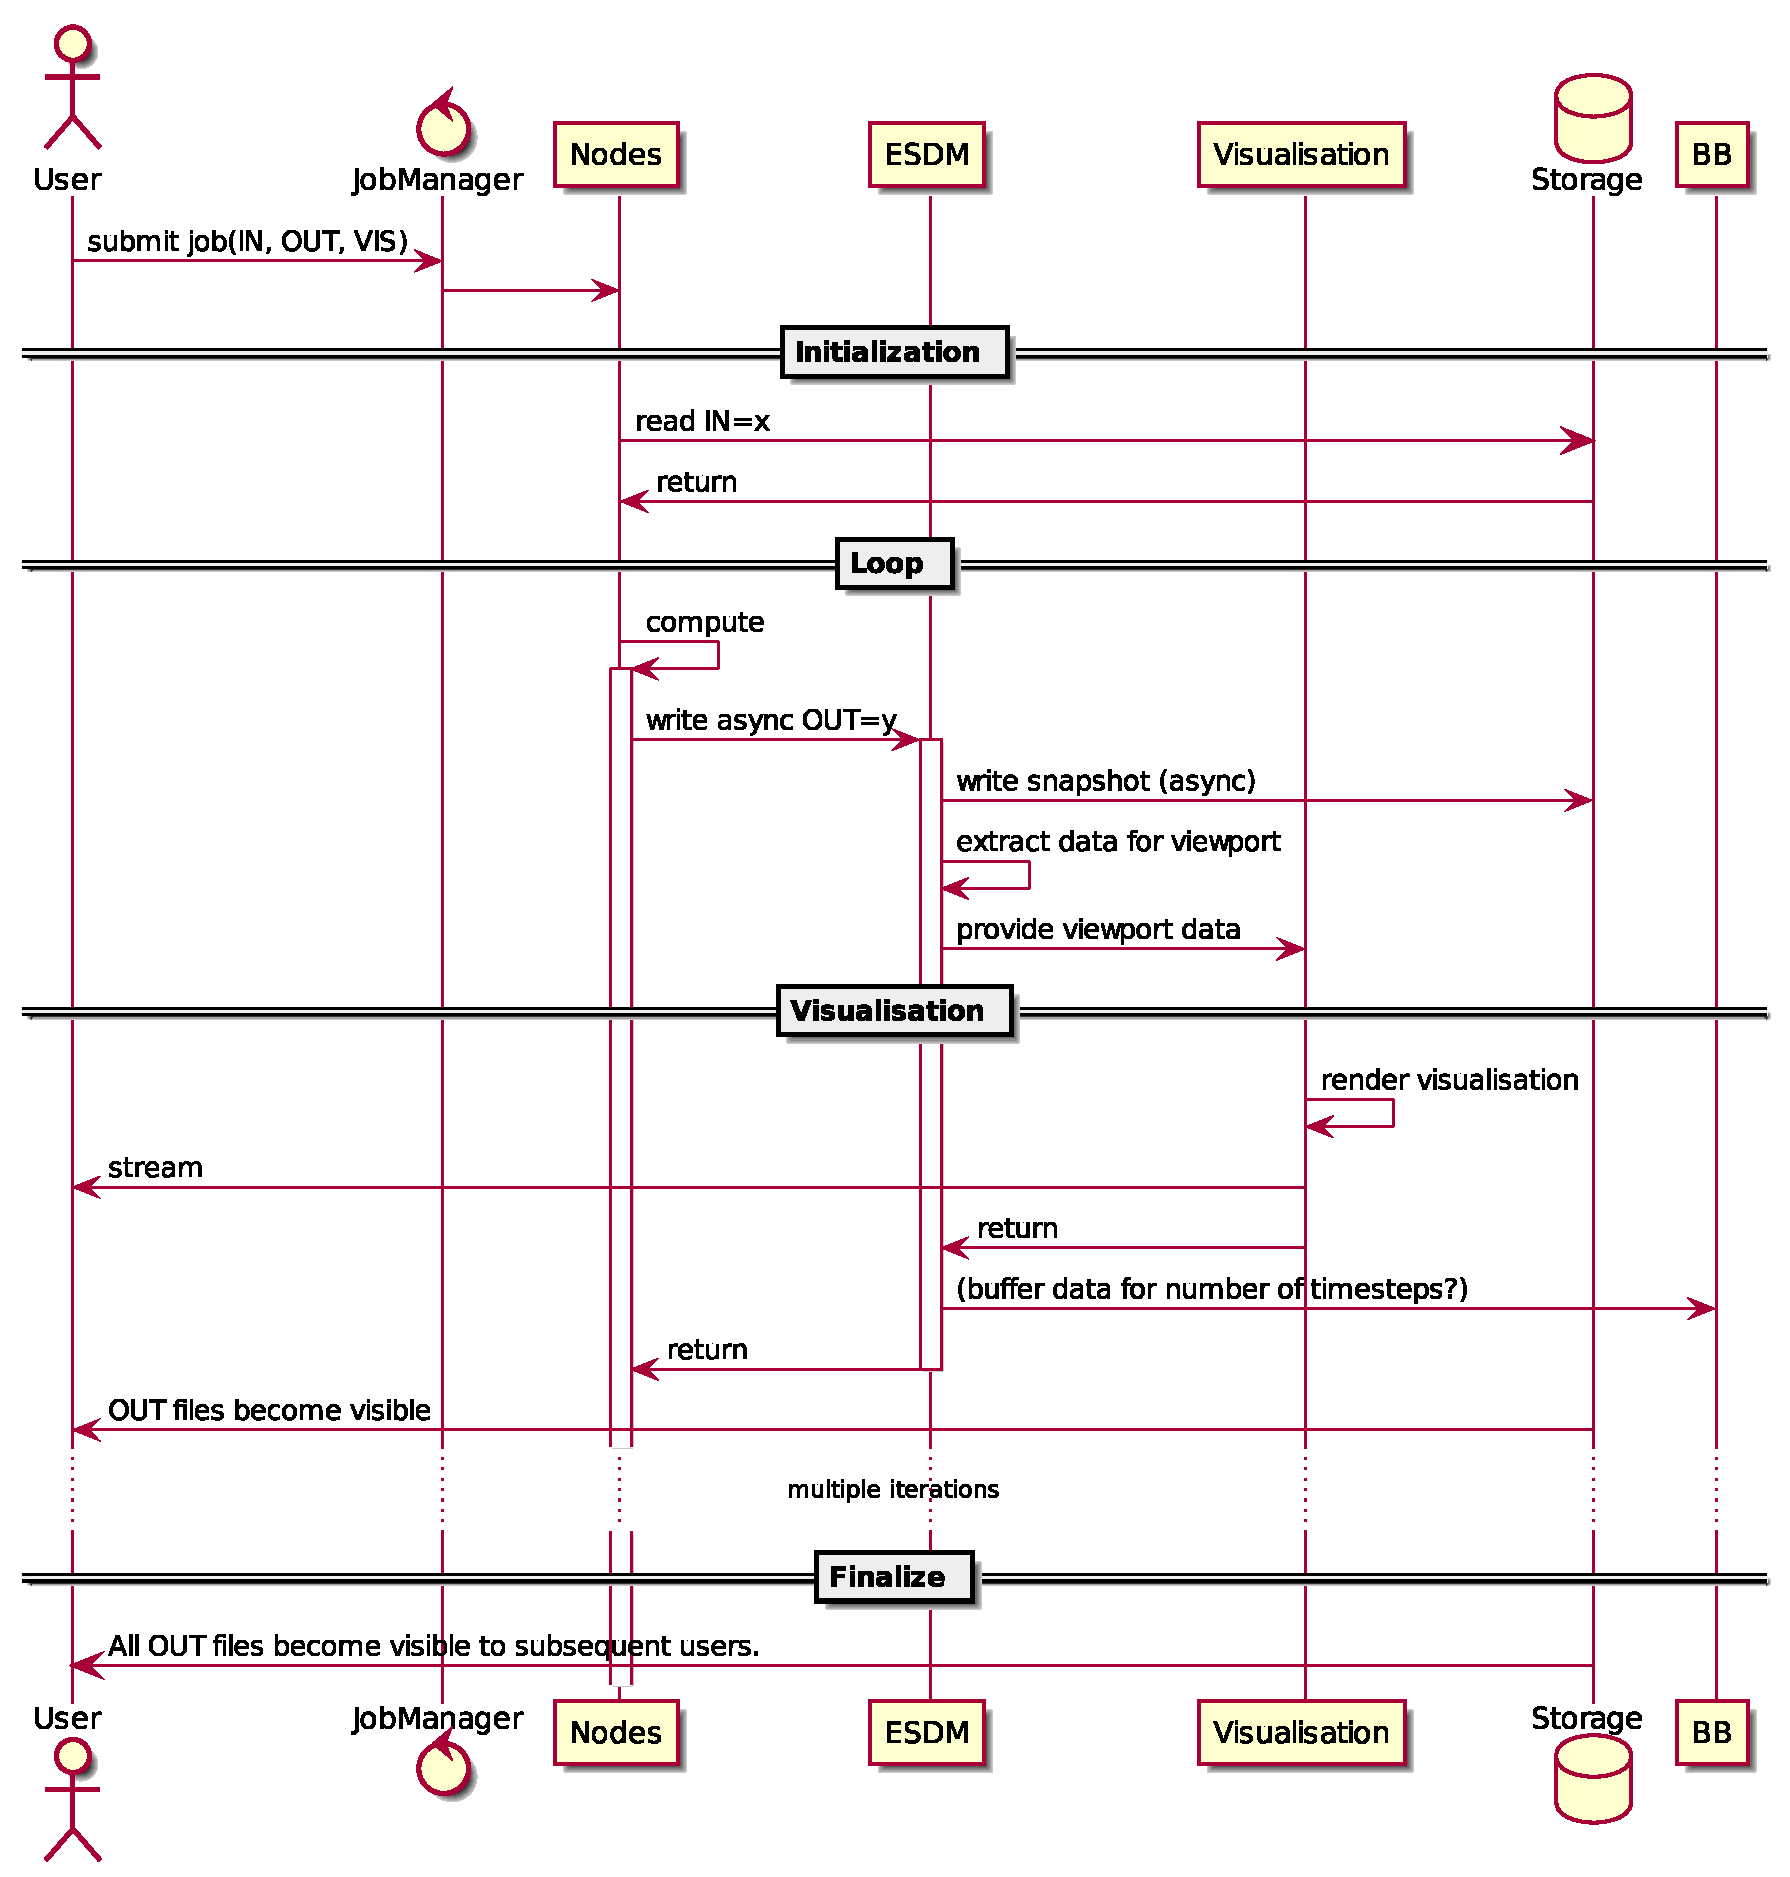
\includegraphics[width=\linewidth]{esdm-fuse/sequence.eps}
	\caption{The simplest approach to expose data to legacy applications by creating actual HDF5 files on the fly and cache them on a file system.}
	\label{fig:fuse hdf5 sequence}
\end{figure}



%%%%%%%%%%%%%%%%%%%%%%%%%%%%%%%%%%%%%%%%%%%%%%
\subsection{Process View}


\begin{figure}
	\centering
	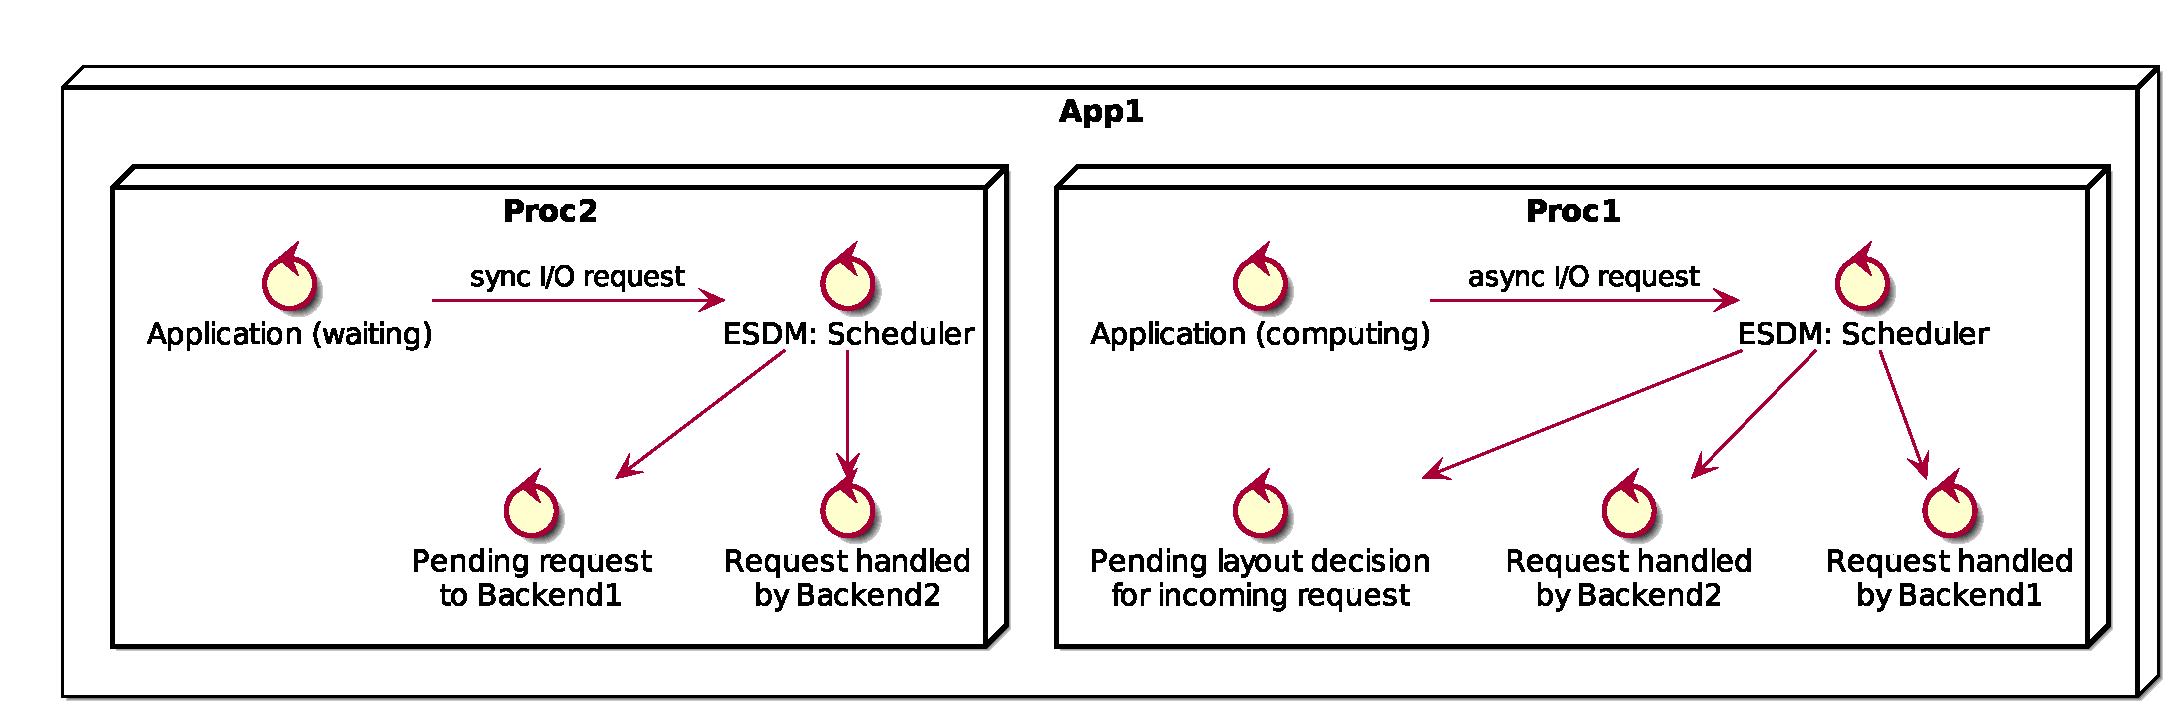
\includegraphics[width=\linewidth]{esdm-fuse/process.eps}
	\caption{Process view to a FUSE legacy backend for ESDM. Application browsers a FUSE file systems which are generated based on the available metadata. As the application opens a file, the ESDM creates an HDF5 file which can be then read just a usual HDF5 file.}
	\label{fig:esdm fuse process view}
\end{figure}

Following the reasoning in \Cref{sec: fuse/development} HDF5 files would need to be generated and stored before file access requests can be handled.
\Cref{fig:esdm fuse process view} separates the process of accessing an available file and the actual generation of the file.
If the application is already running and the requests HDF5 file is not already present, the reconstruction can be performed on the node of the application.
If the application is not yet running, the scheduler could start a reconstruction before the application is started.
In both cases, a component that generates the HDF5 file is required which is represented by the ESDM HDF5 Creator.







%%%%%%%%%%%%%%%%%%%%%%%%%%%%%%%%%%%%%%%%%%%%%%
\subsection{Physical View}

\begin{figure}
	\centering
	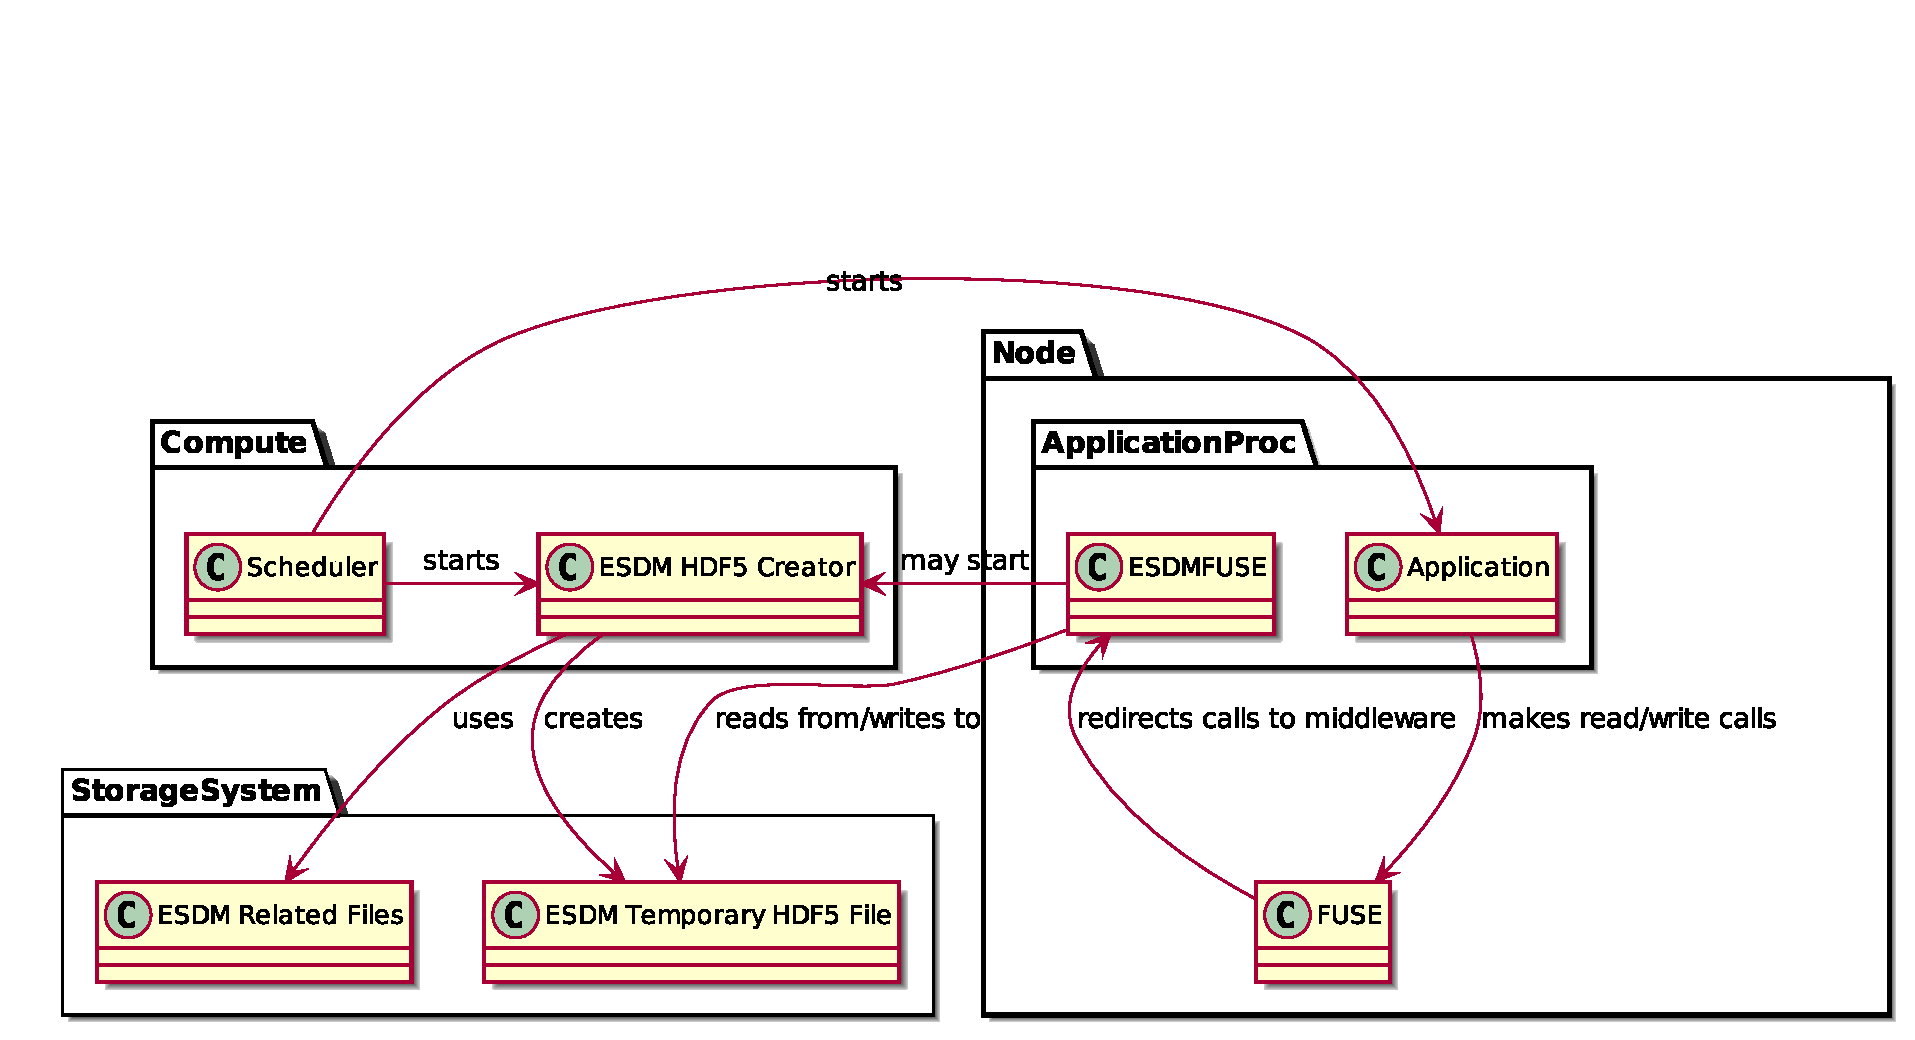
\includegraphics[width=\linewidth]{esdm-fuse/physical.eps}
	\caption{Physical View: Allow legacy applications to access data stored to ESDM by creating HDF5 on the fly or by scanning job files in advance.}
	\label{fig:esdm fuse physical view}
\end{figure}

The provision of a FUSE legacy interface allows for several different deployment models.
\Cref{fig:esdm fuse physical view} illustrates where the ESDM FUSE related component would be active within the data centre.
To require only little modifications and exploit independent data access FUSE is assumed to be available on the compute nodes.
The scheduler may be modified to start the ESDM HDF5 Creators before spawning a job.
The actual ESDM data, as well as temporary HDF5 files, would be stored and distributed across multiple storage systems.
